%!TEX root = ../intro.tex
%******************************
%	 Sources of expression noise
%*****************************

\section{Sources of expression noise} 

\cor{Molecular phenotypic variability} across homogeneous populations of cells \cor{can arise} from intrinsic and extrinsic noise, \cor{and deterministic components} (see \textbf{Box 1} on page \pageref{box1}). 
While intrinsic noise is promoter-specific and therefore induces uncoordinated variation in RNA or protein expression between individual genes, extrinsic noise globally influences gene expression across multiple cells and therefore leads to co-variation across larger sets of genes. 
Here, I give an overview on the different sources of intrinsic and extrinsic noise in a variety of biological systems.

\subsection{Intrinsic noise}

Intrinsic noise in cell populations arises from stochasticity in biochemical reactions that lead to the synthesis of mRNAs (transcription) and proteins (translation) within individual cells. 
Regulatory features on the genomic, epigenetic, transcriptional and translational level influence \cor{and control} the strength of intrinsic noise (for an overview see \textbf{Fig.~\ref{fig0:overview_intrinsic}}).

\begin{figure}[!h]
\centering
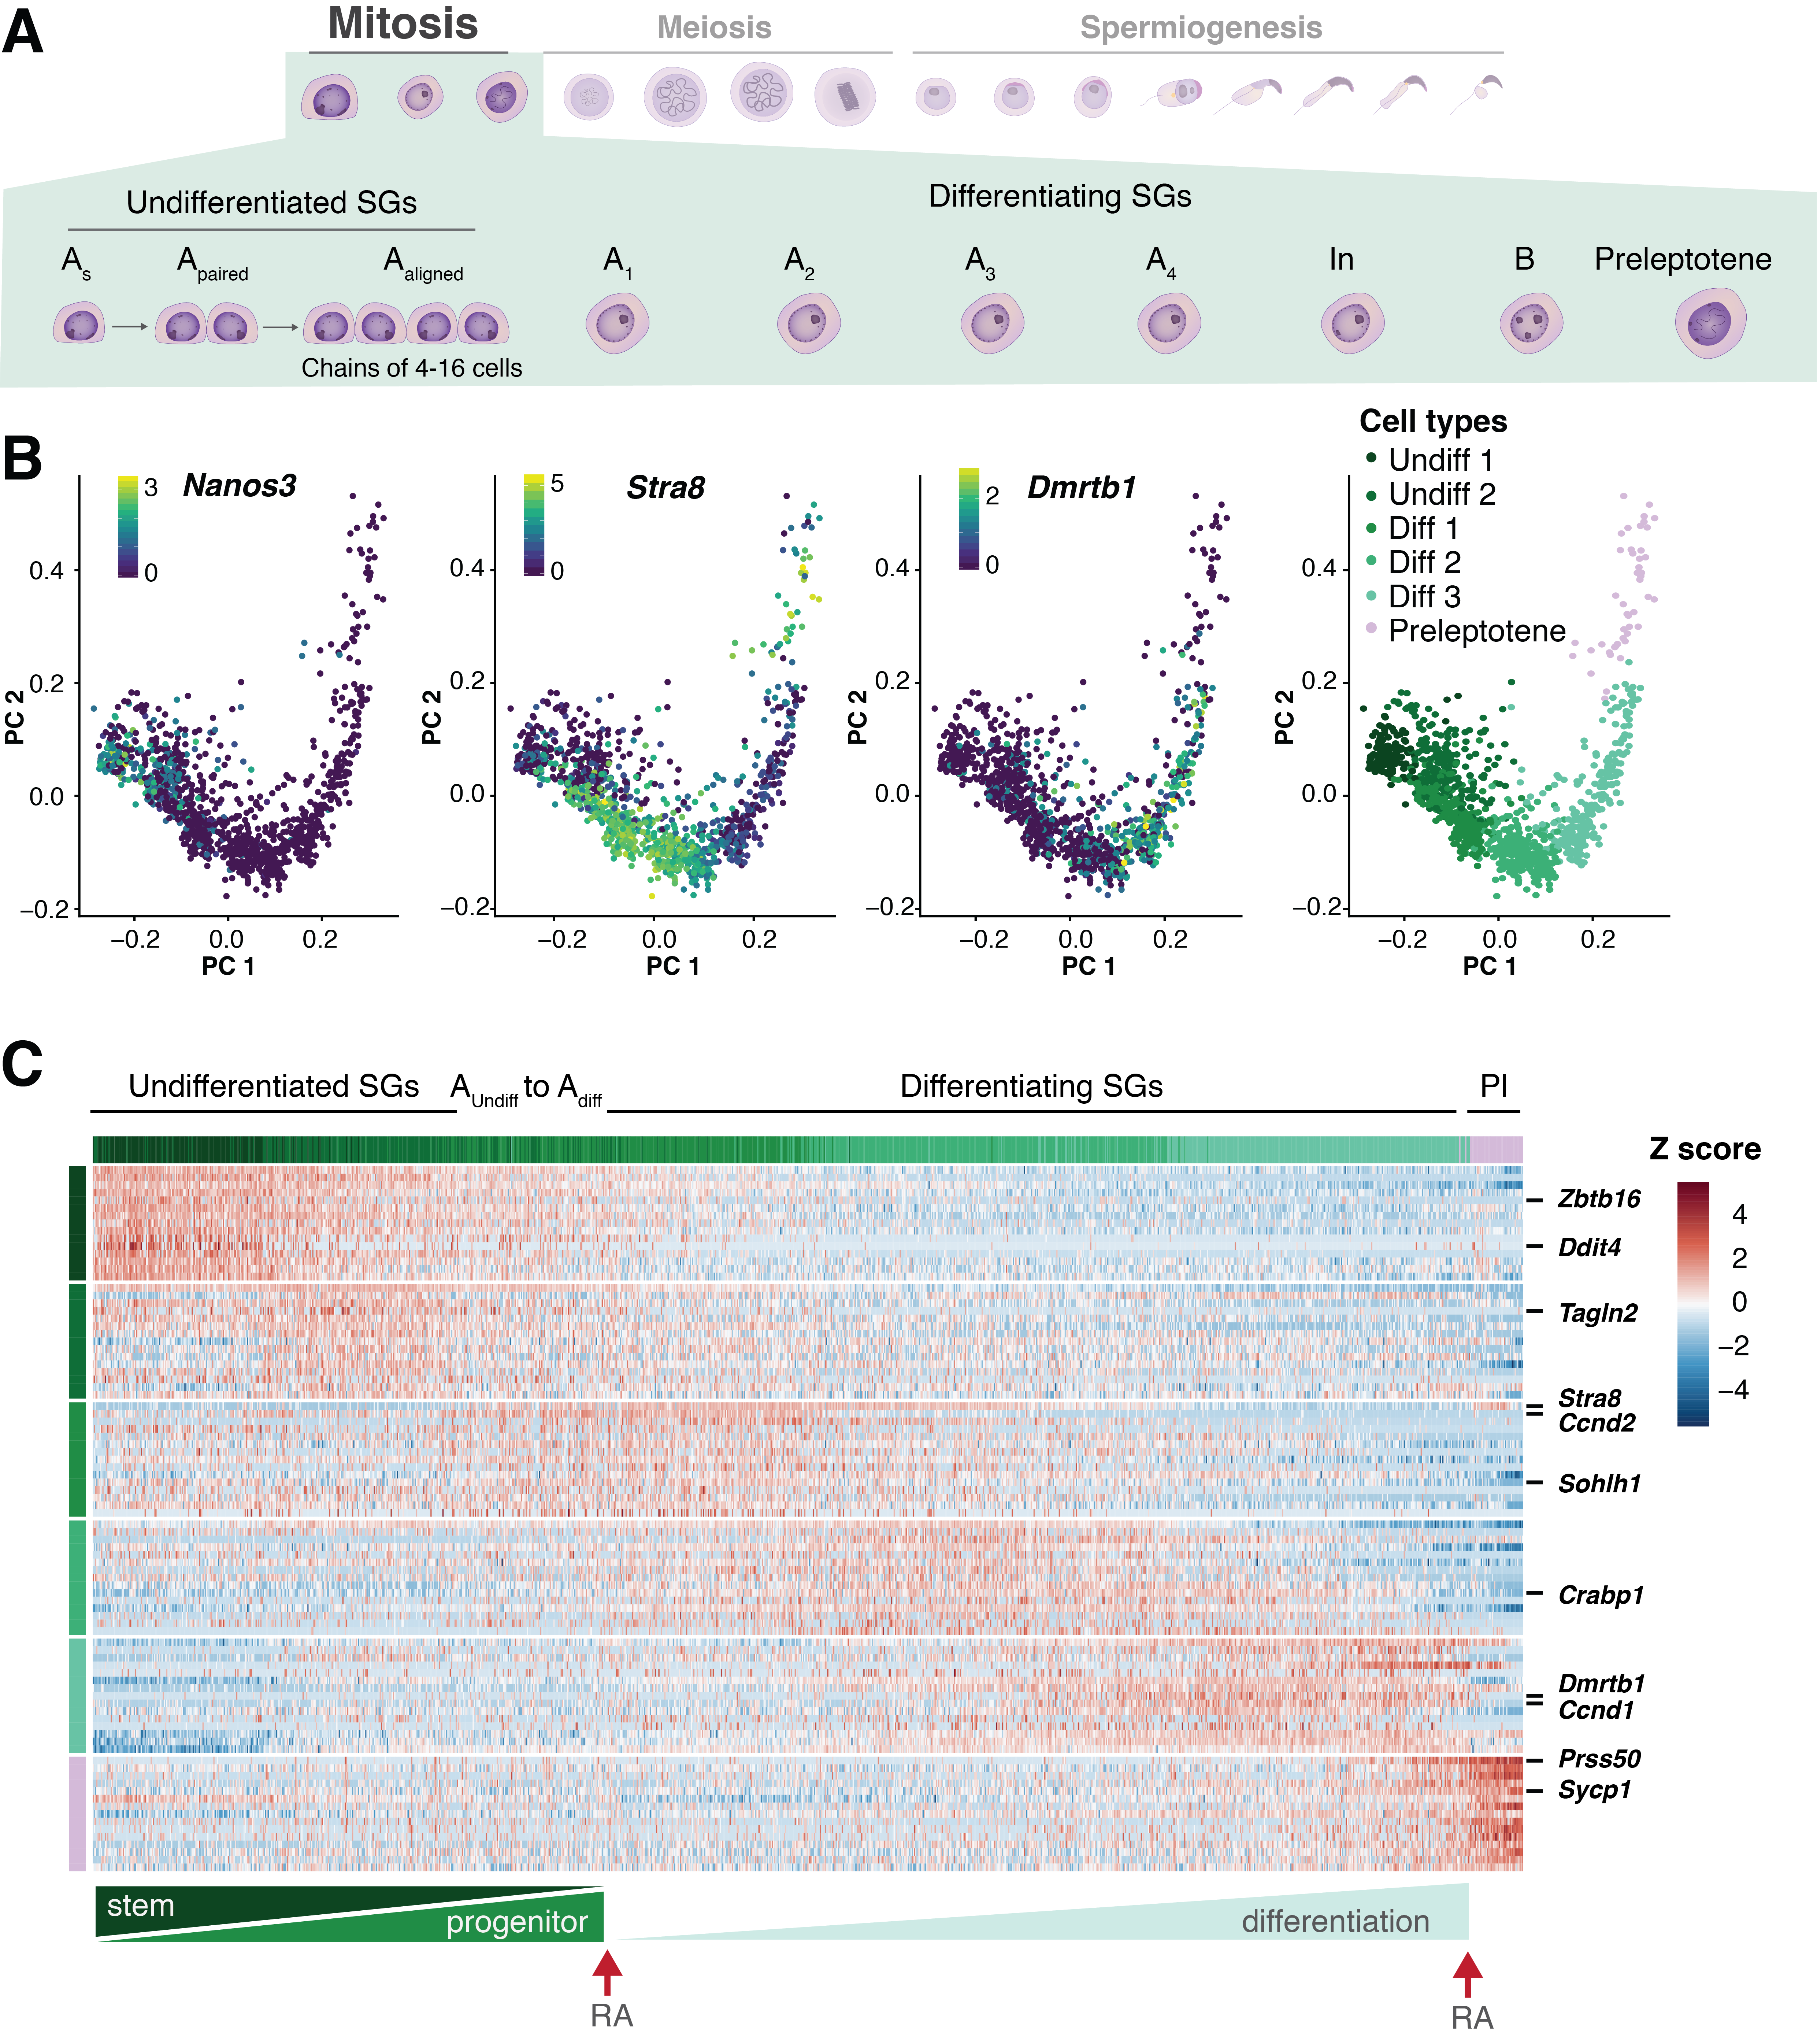
\includegraphics[width=\textwidth]{Fig_6.png}
\caption[Regulatory features that modulate expression noise]{\textbf{Regulatory features that modulate expression noise.}\\
Promoter sequence, number of transcription factor (TF) binding sites (TFBS), number of transcriptional start sites (TSS), enhancer elements, RNA polymerase II (RNAPII) loading, DNA methylation, nucleosome positioning, histone modifications, polycomb repressive complex binding, \glspl{miRNA}, nuclear export of mRNA, ribosome binding and blockage via stem loop formation are features that induce gene-specific intrinsic noise.}
\label{fig0:overview_intrinsic}
\end{figure}

\subsubsection{DNA features}

One of the key regulatory steps prior to RNA synthesis is the binding of \glspl{TF} to specific DNA sequences within the regulatory region (promoter) of a gene which then triggers the controlled production of primary RNA transcripts from the DNA of this gene \citep{Latchman1997}. 
Mutations in the DNA sequence such as \glspl{SNV} can alter the binding affinity of TFs and therefore the rate at which a gene is expressed \textbf{(Fig.~\ref{fig0:DNA_features})}. 
A systematic study of the \gls{TDH3} gene expression in yeast found that mutations in known \glspl{TFBS} decrease mean expression and increase expression noise. 
Moreover, Metzger \textit{et al.}, 2015 \cor{proposed} that evolutionary selection removes mutations that increase expression noise and that SNVs with large effects on expression noise show the lowest frequency within sampled yeast strains \citep{Metzger2015}. 
\cor{However, this examined one promoter in stable environmental conditions. 
How selection on mutations that induce variability in expression works in more complex systems and across multiple promoters is still unexplored.}\\

One of the most widely studied DNA motifs in relation to transcriptional noise is the TATA-box motif in promoters. 
Generally, TATA-box containing promoters show high levels of transcriptional noise \textbf{(Fig.~\ref{fig0:DNA_features})} \citep{Faure2017}, possibly due to a simple activation cycle containing one or few inactive states \citep{Zoller2015}. 
Moreover, TATA-box containing genes show an increased interspecies variability \citep{Tirosh2006} and higher spontaneous mutational variation \citep{Landry2007}, indicating an increased evolvability of these particular genes. 
In an early study, Raser \textit{et al.}, 2004 studied the noisy expression controlled by the budding yeast \gls{PHO5} promoter. 
This promoter contains the TATA-box motif and it has been shown that transcriptional noise is reduced when a mutational modification decreases the TATA-box strength \citep{Raser2004}. 
A more recent study confirmed this result and found mutations in yeast promoters that eliminate the TATA-box motif which lead to reduced noise levels for these genes \citep{Hornung2012}. 
\cor{The TATA-box is therefore one genomic feature that can differentiate between genes with variable and stable expression. Gene expression instability can endow cells with the ability to rapidly respond to environmental changes. 
TATA-box motifs are enriched amongst stress response genes, which support their role in early adjustment to changing environmental conditions\citep{Lopez-Maury2009}.}\\

\cor{However, a} possible confounding factor for the increased noise of TATA-box containing promoters is the number of TFBSs. 
Tirosh \textit{et al.}, 2006 detected a two-fold enrichment of TFBSs in TATA-box containing promoters \citep{Tirosh2006}. 
A later study showed that transcriptional noise scales with increased numbers of TFBSs \textbf{(Fig.~\ref{fig0:DNA_features})} \citep{Sharon2014}. 
Furthermore, TATA-box containing genes lack enhancing histone marks and their increased variability in expression can therefore be explained by repressed chromatin \citep{Choi2008} (see \textbf{Section \ref{sec0:epigenetic}}).  

\begin{figure}[!h]
\centering
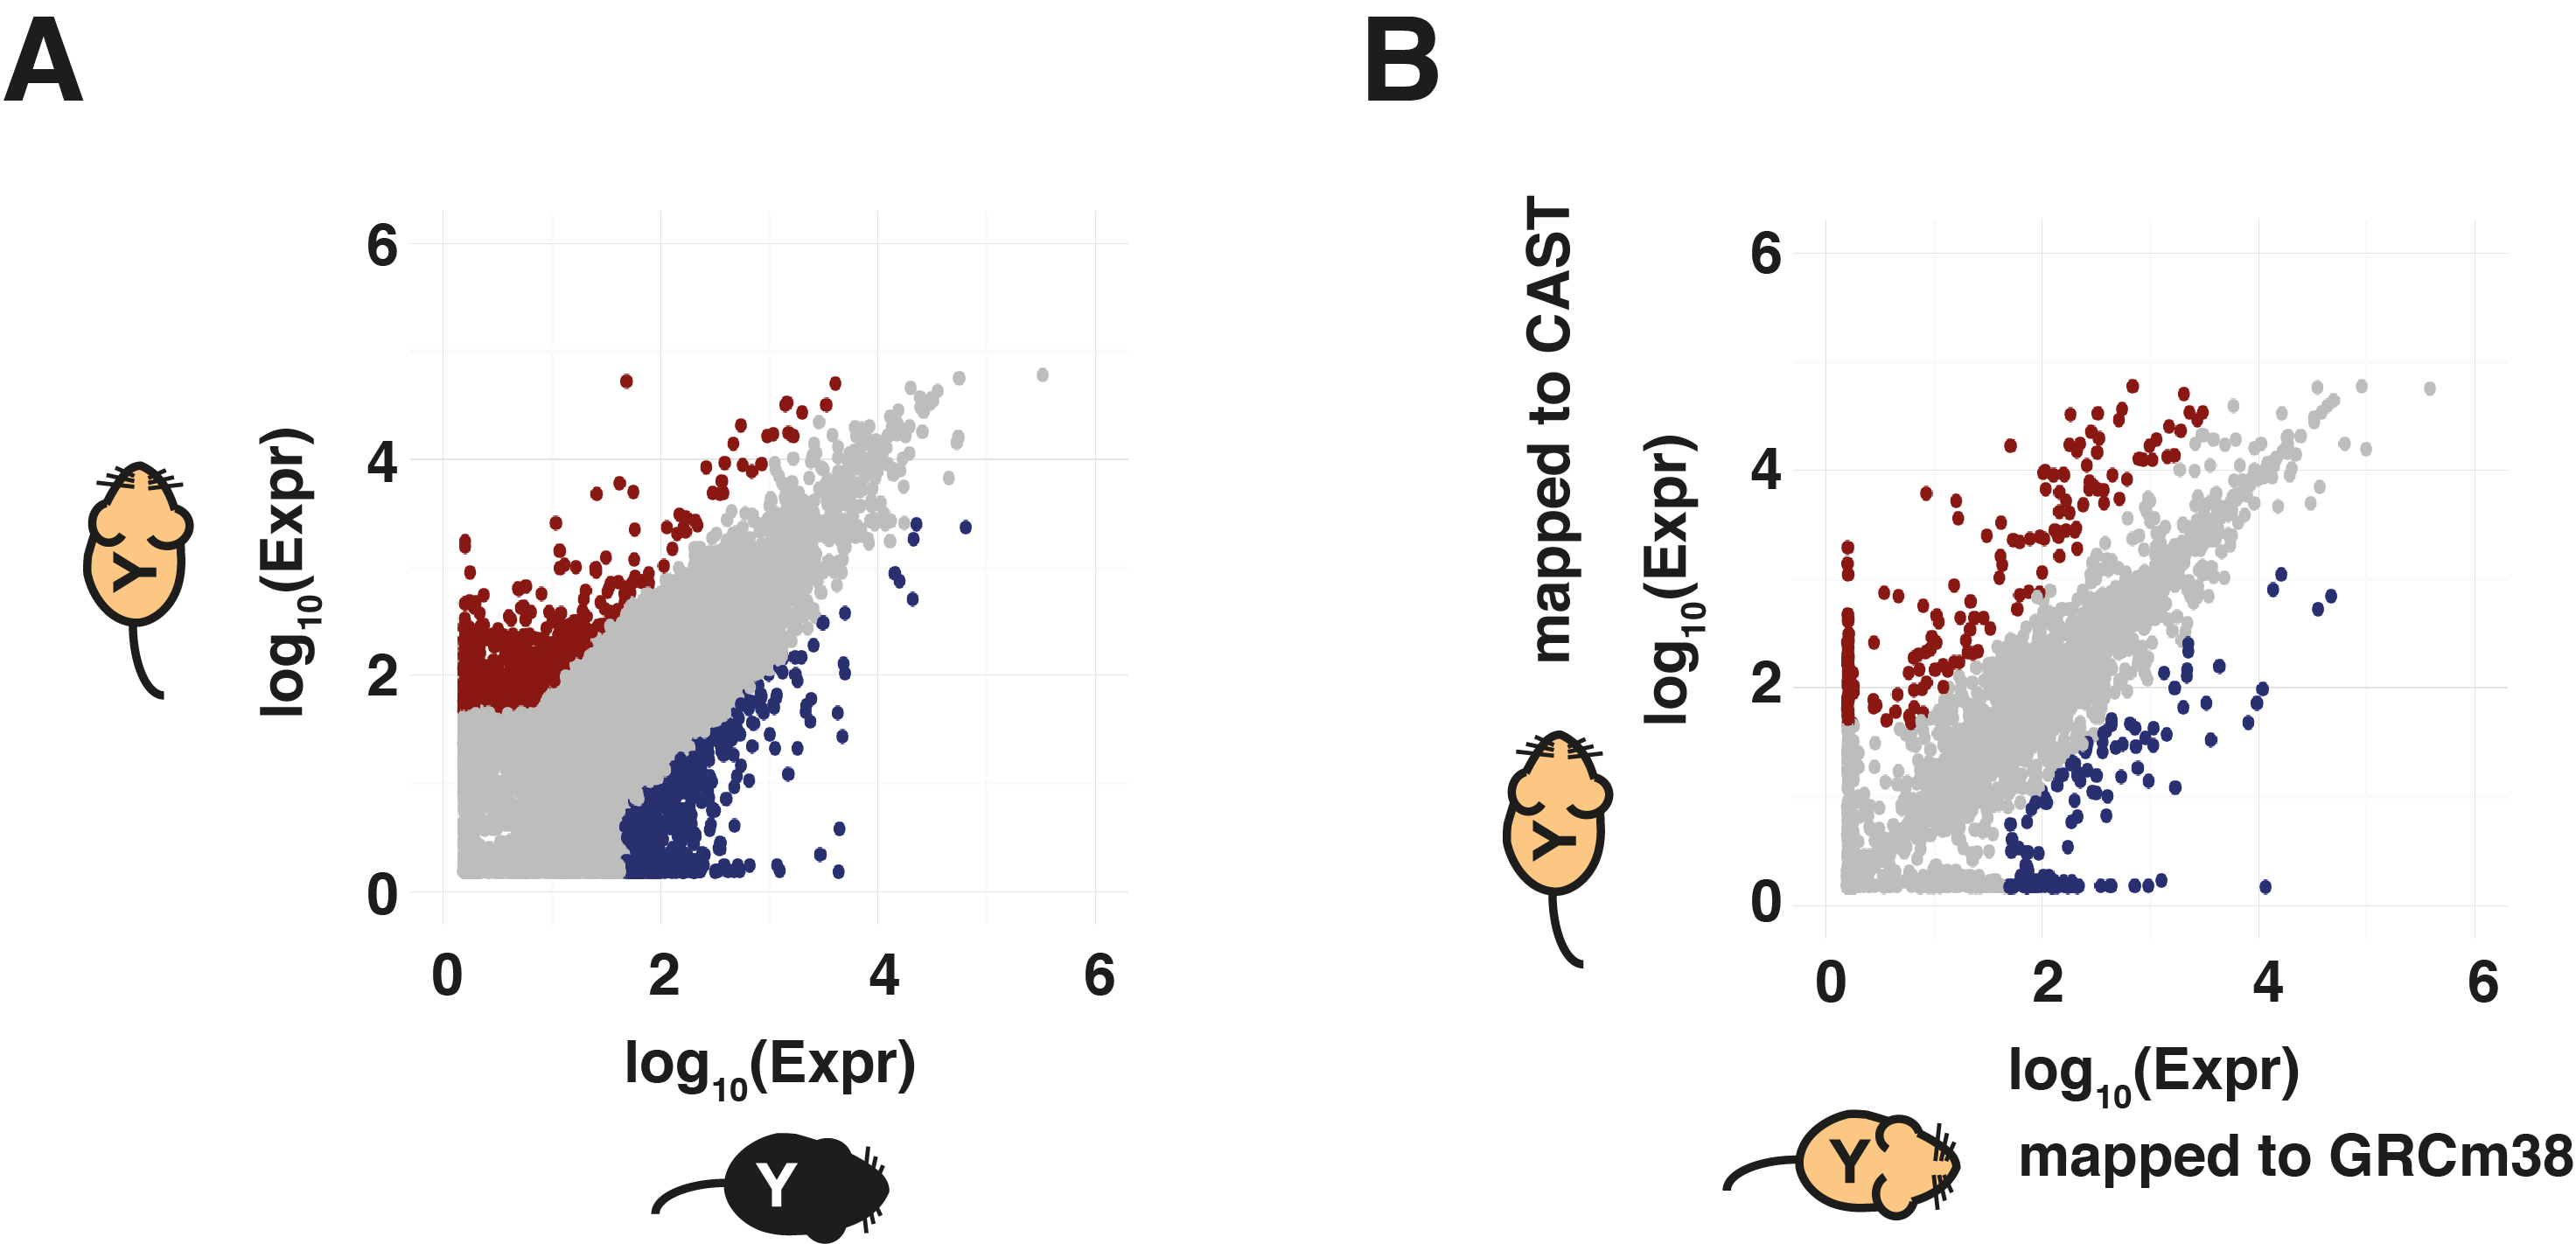
\includegraphics[width=\textwidth]{Fig_7.png}
\caption[Features of the DNA sequence induce expression noise]{\textbf{Features of the DNA sequence induce expression noise.}\\
Mutations of the transcription factor (TF) binding site (TFBS), the presence of a TATA box, increase number of TFBSs, reduced number of transcriptional start sites (TSSs) and reduced copy number of genes can induce transcriptional noise.}
\label{fig0:DNA_features}
\end{figure}

Promoters can be classified based on their shape as narrow, with few \glspl{TSS} that predominantly control tissue-specific gene expression, and broad promoters with larger numbers of TSSs that control the expression of house keeping genes. 
Mutations that alter the shape of promoters increase transcriptional \cor{variability} \citep{Schor2017a}. 
Furthermore, promoters with one or few TSS show higher levels of expression variability \textbf{(Fig.~\ref{fig0:DNA_features})} \citep{Faure2017}.\\

In addition to \glspl{SNV}, \glspl{CNV} (usually defined as copy number variability of regions $\geq$ 1kb in comparison to a reference genome) in parts of the genome influence gene expression and contribute to, for example, schizophrenia and autism \citep{Gamazon2015}. 
Combined analysis of DNA and RNA has shown that genes with low copy number tend to be more noisily expressed compared to genes encoded by multiple copies \textbf{(Fig.~\ref{fig0:DNA_features})} \citep{Dey2015}. 
In the context of monoallelic expression, genes located on the X chromosome show increased mRNA half-life which in turn increases transcript stability and reduces noise to levels of autosomal genes \citep{Faure2017}.

\cor{In sum, these findings highlight that multiple correlated genomic features are associated with modulating noise. 
While most studies focused on linking individual genomic features to changes in expression variability, it is not possible to disentangle the individual underlying sources of transcriptional variability. }

\subsubsection{Epigenetic factors}
\label{sec0:epigenetic}

Epigenetic research is defined as "the study of changes in gene function that are mitotically and/or meiotically heritable and that do not entail a change in DNA sequence" \citep{Wu2001}. 
Epigenetic factors are generally described as DNA methylation at \gls{CpG} dinucleotides, histone modifications and nucleosome positioning  \citep{Portela2010}. 
\textbf{Table \ref{tab0:epigenetic}} summarises the relationship between epigenetic features and \cor{variable} gene expression. \\

\Gls{CGI} are genomic sites of more than 200 bases with a GC content of more than 50\% and are usually unmethylated. 
Methylation of CGIs in promoters is linked to gene silencing while DNA methylation in gene bodies facilitates transcription \citep{Portela2010}.  
Recently, the presence of CGIs in gene bodies but also at the TSS and in promoter regions was linked to a reduction in transcriptional \cor{variability} \citep{Faure2017}. 
\cor{Morgan and Marioni, 2018 further distinguished between genes promoters associated with short and long CGIs.  
Similar to the presence of TATA-box motifs as described above, the length of CGIs in promoter regions controls how variably a gene is expressed. 
Genes associated with short CGIs tend to be more variably expressed and allow an early response to stimulation, exemplified by observations in mouse bone-marrow derived dendritic cells and human breast cancer cells \citep{Morgan2018}.
However, it is not clear whether the length of CGIs is the sole driver for variable gene expression or how multiple genomic features work together to induce transcriptional variability.} \\

Modifications of histones induce the \cor{opening} or repression of chromatin and  therefore indirectly modulate gene expression \citep{Suganuma2011}. 
In an extensive study to link histone modifications to transcriptional \cor{variability}, Faure \textit{et al.}, 2017 detected several histone modifications in promoter/core promoter motifs, at the TSS and in gene bodies that increase or decrease \cor{variability}. 
The repressive \gls{H3K27me3} mark is linked to higher \cor{variability} when present at the TSS, in promoters and in gene bodies. 
The enhancer related \gls{H3K4me1} mark only increases \cor{variability} when present at the TSS and in the core promoter sequence while the repressive \gls{H3K9me3} mark increases \cor{variability} when present in the promoter motif. 
The activating marks \gls{H3K4me3}, \gls{H3K9ac} and \gls{H3K36me3} are linked to low levels of \cor{variability} when present in gene bodies. 
In addition to these single features, bivalent promoters that carry the repressive \gls{H3K27me3} and enhancing \gls{H3K4me3} marks show high levels of transcriptional \cor{variability} \citep{Faure2017}.
\cor{Here and in Morgan and Marioni, 2018, the authors profiled molecular phenotypic variability in "homogeneous" populations of glspl{mESC} as proxy for transcriptional noise.
While the effect of fluctuation in cell-cycle stages was regressed out, unobserved variation in, for example, the differentiation potential of mESCs in serum grown medium\cite{Kolodziejczyk2015cell} could still exist.
It is therefore difficult to use scRNA-Seq data to study the true underlying effect of transcriptional noise on the overall observable phenotypic variability.}\\ 

\cor{One suggestion why bivalent promoters show high transcriptional variability was brought forward by Kar \emph{et al.}, 2017.
Here, the authors studied the function of \glspl{PRC} in mESCs.}
PRCs are epigenetic modifiers of histones that repress transcription of developmental genes \citep{Chittock2017} and they can bind together with active \gls{RNAPII} to bivalent promoters. 
Switching between the repressed and active states introduces gene expression variability across a population of cells \cite{Kar2017}.
\cor{However, bulk measures were used to identify the bivalency of promoters.
That leaves the possibility that in a fraction of cells the promoter resides in an open state while in other cells the promoter is repressed. 
This highlights the fact that bulk measures are not suitable to obtain a correct measure of promoter states in cell populations that could contain unobserved cell state heterogeneity.} 

Chromatin is the packaged state of DNA within the nucleus and its central elements are nucleosomes. 
Nucleosomes are combinations of eight of the four histones (H3, H4, H2A, H2B) around which 147 bases of DNA twist. 
An array of histone modifying enzymes exist that regulate the opening or closing of the chromatin; termed heterochromatin and euchromatin, respectively \citep{Kouzarides2007}. 
Tirosh \textit{et al.}, 2008 showed that promoters with high nucleosome occupancy close to the TSS tend to display a high range of expression levels across varying conditions (transcriptional plasticity). 
Distant nucleosome-rich regions are on the other hand associated with low transcriptional \cor{variability} \citep{Tirosh2008}. 
Nucleosome covered promoters display shorter transcriptional rates, which in turn explains increased transcriptional \cor{variability} for these promoters \cite{Dey2015}. 
Single-cell measures indicate cell-to-cell variations in nucleosome positioning around the \textit{PHO5} promoter upon stress induction. 
Even in the non-stressed state, a small fraction of cells exhibit nucleosome free regions at the promoter which explains low and possibly noisy expression of \textit{PHO5} \citep{Small2014}.
\cor{This observation again highlights the lack of resolution when using bulk measures to profile the promoter architectures in cell populations.
However, current single-cell technologies to profile epigenetic marks lack throughput and are influenced by high levels of technical noise.
The observed variations in nucleosome occupancy could therefore be driven by technical variation.} 
 
\newpage

Boundaries between heterochromatin and euchromatin are controlled by boundary elements, such as the transcription factor \Gls{CTCF}, that recruit chromatin modifying factors \citep{Kouzarides2007}. 
CTCF also regulates transcription by activating or repressing promoters and regulates distant chromatin interactions \citep{Kim2015a}. 
Recent studies suggest that long-range enhancer-promoter interactions modulate transcriptional noise. 
Interference of CTCF-mediated enhancer-promoter contact either by CTCF knock-out or CTCF-binding site deletion leads to increased expression variability in selected genes \citep{Ren2017}. 
\cor{This study however only profiled protein abundance of few genes and did not correct for changes in mean expression that are highly correlated with changes in variance \cite{Brennecke2013}.}
Enhancers are cis-regulatory elements of non-coding DNA containing TFBSs that regulate the expression of neighbouring genes \citep{Blackwood1998}. 
Genes within super-enhancer loci, a region with multiple enhancers, control pluripotency master regulators and show high levels of variability in expression down-stream targets of these master regulators show similar co-variation across mESCs \citep{Faure2017}.

\begin{table}[hb	]
\centering
\caption{Epigenetic control of transcriptional noise}
\label{tab0:epigenetic}
\begin{tabular}{l l c c}
\toprule
\toprule
 & Feature & \cor{Variable} & Stable \\ 
\midrule
\midrule
\multirow{3}{*}[-2pt]{DNA methylation} & CGIs &  & \checkmark{} \\
\cmidrule{2-4}
& Short CGIs & \checkmark{} &  \\
\cmidrule{2-4}
& Gene body methylation &  & \checkmark{} \\
\midrule
\multirow{7}{*}[-2pt]{Histone modification} & H3K27me3 (TSS, promoter, gene body) & \checkmark{}  & \\
\cmidrule{2-4}
& H3K4me1 (TSS, promoter) & \checkmark{}  & \\
\cmidrule{2-4}
& H3K9me3 (promoter) & \checkmark{}  & \\
\cmidrule{2-4}
& H3K4me3 (gene bodies) &  & \checkmark{}\\
\cmidrule{2-4}
& H3K9ac (gene bodies) &  & \checkmark{} \\
\cmidrule{2-4}
& H3K36me3 (gene bodies) &  & \checkmark{} \\
\cmidrule{2-4}
& H3K27me3 and H3K4me3 & \checkmark{}  & \\
\midrule
\multirow{3}{*}[-2pt]{Nucleosome position} & Nucleosome rich promoters & \checkmark{} & \\
\cmidrule{2-4}
& Distant nucleosome rich regions &  & \checkmark{} \\
\cmidrule{2-4}
& Deletion of nucleosome remodelling complexes & \checkmark{}  & \\
\midrule
\multirow{7}{*}[-2pt]{Genome architecture} & CTCF knock-out & \checkmark{} & \\
\cmidrule{2-4}
& CTCF binding site depletion & \checkmark{} & \\
\cmidrule{2-4}
& Clustered genes &  & \checkmark{} \\
\cmidrule{2-4}
& Nuclear-lamina associated genes & \checkmark{} & \\
\bottomrule
\bottomrule
\end{tabular}
\end{table} 

\newpage

Moreover, the positioning of genes on the genome controls expression noise with densely clustered genes being less \cor{variably} expressed in comparison to non-clustered genes \citep{Kustatscher2017}. 
Additionally, genes positioned next to “noisy” genes display higher levels of transcriptional variability compared to genes that are located in proximity to “stable” genes \citep{Kar2017}. 
Expression \cor{variability} is also increased for genes that are located in a repressed neighbourhood, namely active genes in constitutive nuclear lamina-associated domains \citep{Faure2017}.
\cor{This finding again highlights that genes associated with repressed chromatin display higher transcriptional variability compared to genes associated with open chromatin.
Single-cell measures are needed to provide an insight into whether this effect is driven by so called "leaky" expression from closed promoters of if heterogeneous promoter states can be observed.}

\subsubsection{Transcriptional features}

Transcription is initiated by TFs binding to specific regulatory DNA sequences followed by recruitment of RNAPII and RNA synthesis. 
As discussed above, promoter architecture, namely the location and accessibility of TFBS and RNAPII binding sites, dictates mean expression and transcriptional \cor{variability}. \\

In bacteria, the intracellular physical distance between TF source and the promoter sequence influences expression variability. 
TF expression proximal to their target genes results in less \cor{variable} expression compared to TF expression which occurs distant to the promoter sequence \citep{Goni-Moreno2017}. 
Once TFs bind to their target sequence, Carey \emph{et al.}, 2013 showed that the mean expression to \cor{expression variability} ratio is promoter dependent while in the majority of cases, \cor{variability} negatively scales with mean expression \citep{Carey2013}. \\

Similar to TF binding dynamics, the assembly of RNAPII complexes modulates transcriptional noise. 
An early study identified the connection between paused RNAPII and synchronous expression of target genes. 
Genes without pre-loaded RNAPII show more stochastic activation patterns \citep{Boettiger2009}. 
This finding has later been confirmed using scRNA-Seq data where increased variability was detected for genes with actively transcribing RNAPII across the full range of expression levels \textbf{(Fig.~\ref{fig0:RNAPII})} \citep{Day2016}.
\cor{However, genes with pre-loaded RNAPII also have a higher CpG content and are depleted for TATA-box elements\cite{Day2016}. 
Once again, the correlation between genomic factors and their individual associations with variation creates a challenge for disentangling their specific effects on molecular phenotypic variation.
Alternatively, this may also represent multiple regulatory layers that combine to modulate noise. }\\

\begin{figure}[!h]
\centering
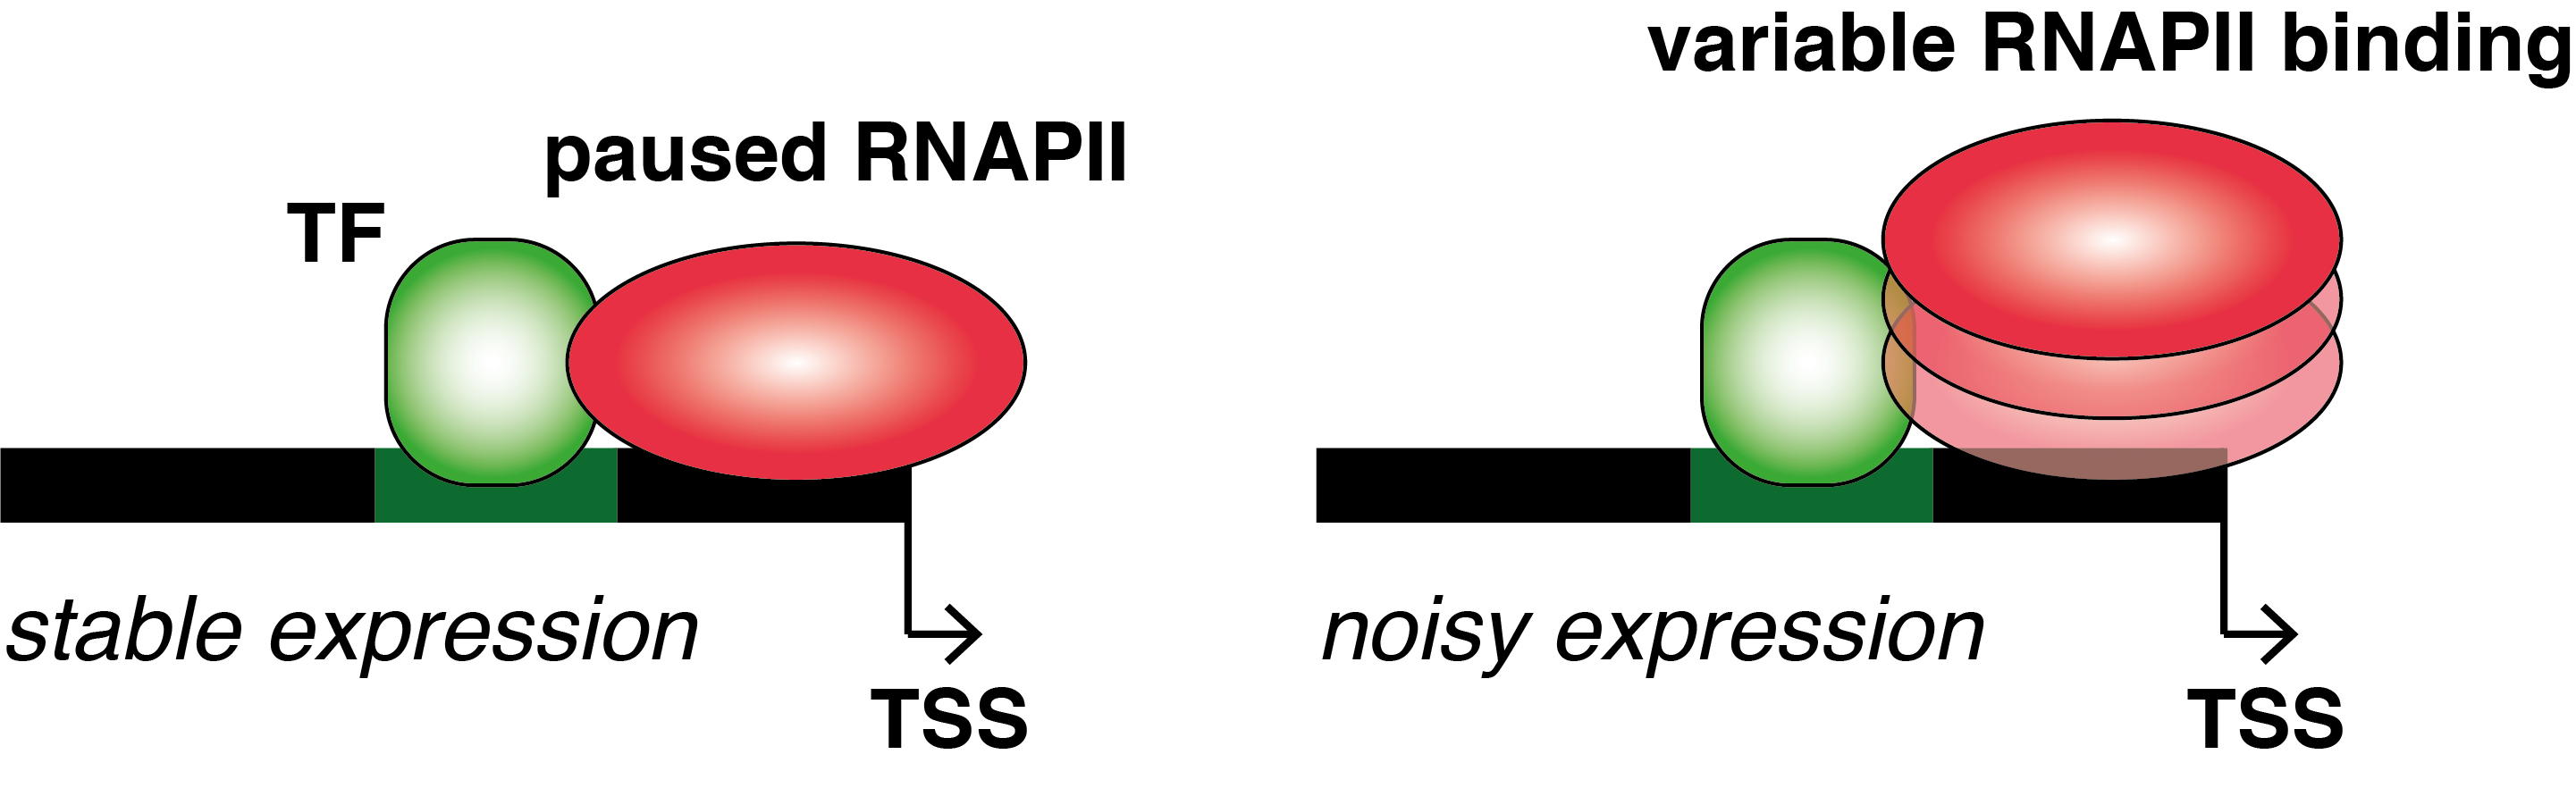
\includegraphics[width=0.7\textwidth]{Fig_8.png}
\caption[RNAPII pausing reduces transcriptional noise]{\textbf{RNAPII pausing reduces transcriptional noise.}\\
Left: Pre-loaded RNA polymerase II (RNAPII) allows direct transcription upon transcription factor (TF) binding. 
Right: RNAPII recruitment induces gene expression variability.}
\label{fig0:RNAPII}
\end{figure} 

\newpage

\subsubsection{Post-transcriptional and translational features}

After synthesis, pre-RNAs are polyadenylated and spliced to form mRNA that relocates from the nucleus to the cytoplasm where translation occurs to synthesise proteins \cite{Glisovic2008}. 
On the post-transcriptional and translational level, mRNA location, structure, degradation and translation have been shown to influence cell-to-cell variation in protein abundance.\\

Upon transcriptional activation, RNAs are produced in burst-like patterns where burst frequency modulates mean expression and noise, and burst size influences solely mean expression \citep{Hornung2012}. 
While bursty transcript synthesis introduces stochastic fluctuations in nuclei between cells, active export of mRNAs into the cytoplasm can dampen this source of variability \textbf{(Fig.~\ref{fig0:posttranscriptional})} \citep{Battich2015a}. 
Reduced cytoplasmic noise has also been shown for two nuclear-retained genes in the mammalian liver. 
Furthermore, this mode of noise control was proposed to be active across a range of metabolic tissues \cite{BaharHalpern2015a}.
\cor{Conversely, a recent study by Hansen \emph{et al.}, 2018 proposed an amplification of transcriptional variability due to nuclear export \cite{Hansen2018}. 
However, the authors computed the Fano factor (variance divided by mean expression) as measure of variability and assumed that its values is not correlated with mean expression. 
This assumption arises from an underlying Poissonian (Fano factor is equal to 1) or over-dispersed Poissonian (Fanor factor is larger than 1) distribution of transcript counts.
In reality, the Fano factor is not constant across the range of mean expression. 
This has been discussed by Gr\"un \emph{et al.}, 2014, who showed scale differences in the coefficient of variation (CV) versus mean expression dependency for lowly and highly expressed genes \cite{Grun2014}.
Hansen \emph{et al.} also showed this effect when plotting the Fano factor versus mean expression.
Across all genes, the cytoplasmic transcript abundance as well as the Fano factor were larger compared to nuclear measures, which is to be expected by the model proposed by Gr\"un \emph{et al.}.
It is therefore recommended to fit a non-parametric curve to variability measure versus mean expression and compare the regression residuals as explained in Chapter 3.}\\

\begin{figure}[!h]
\centering
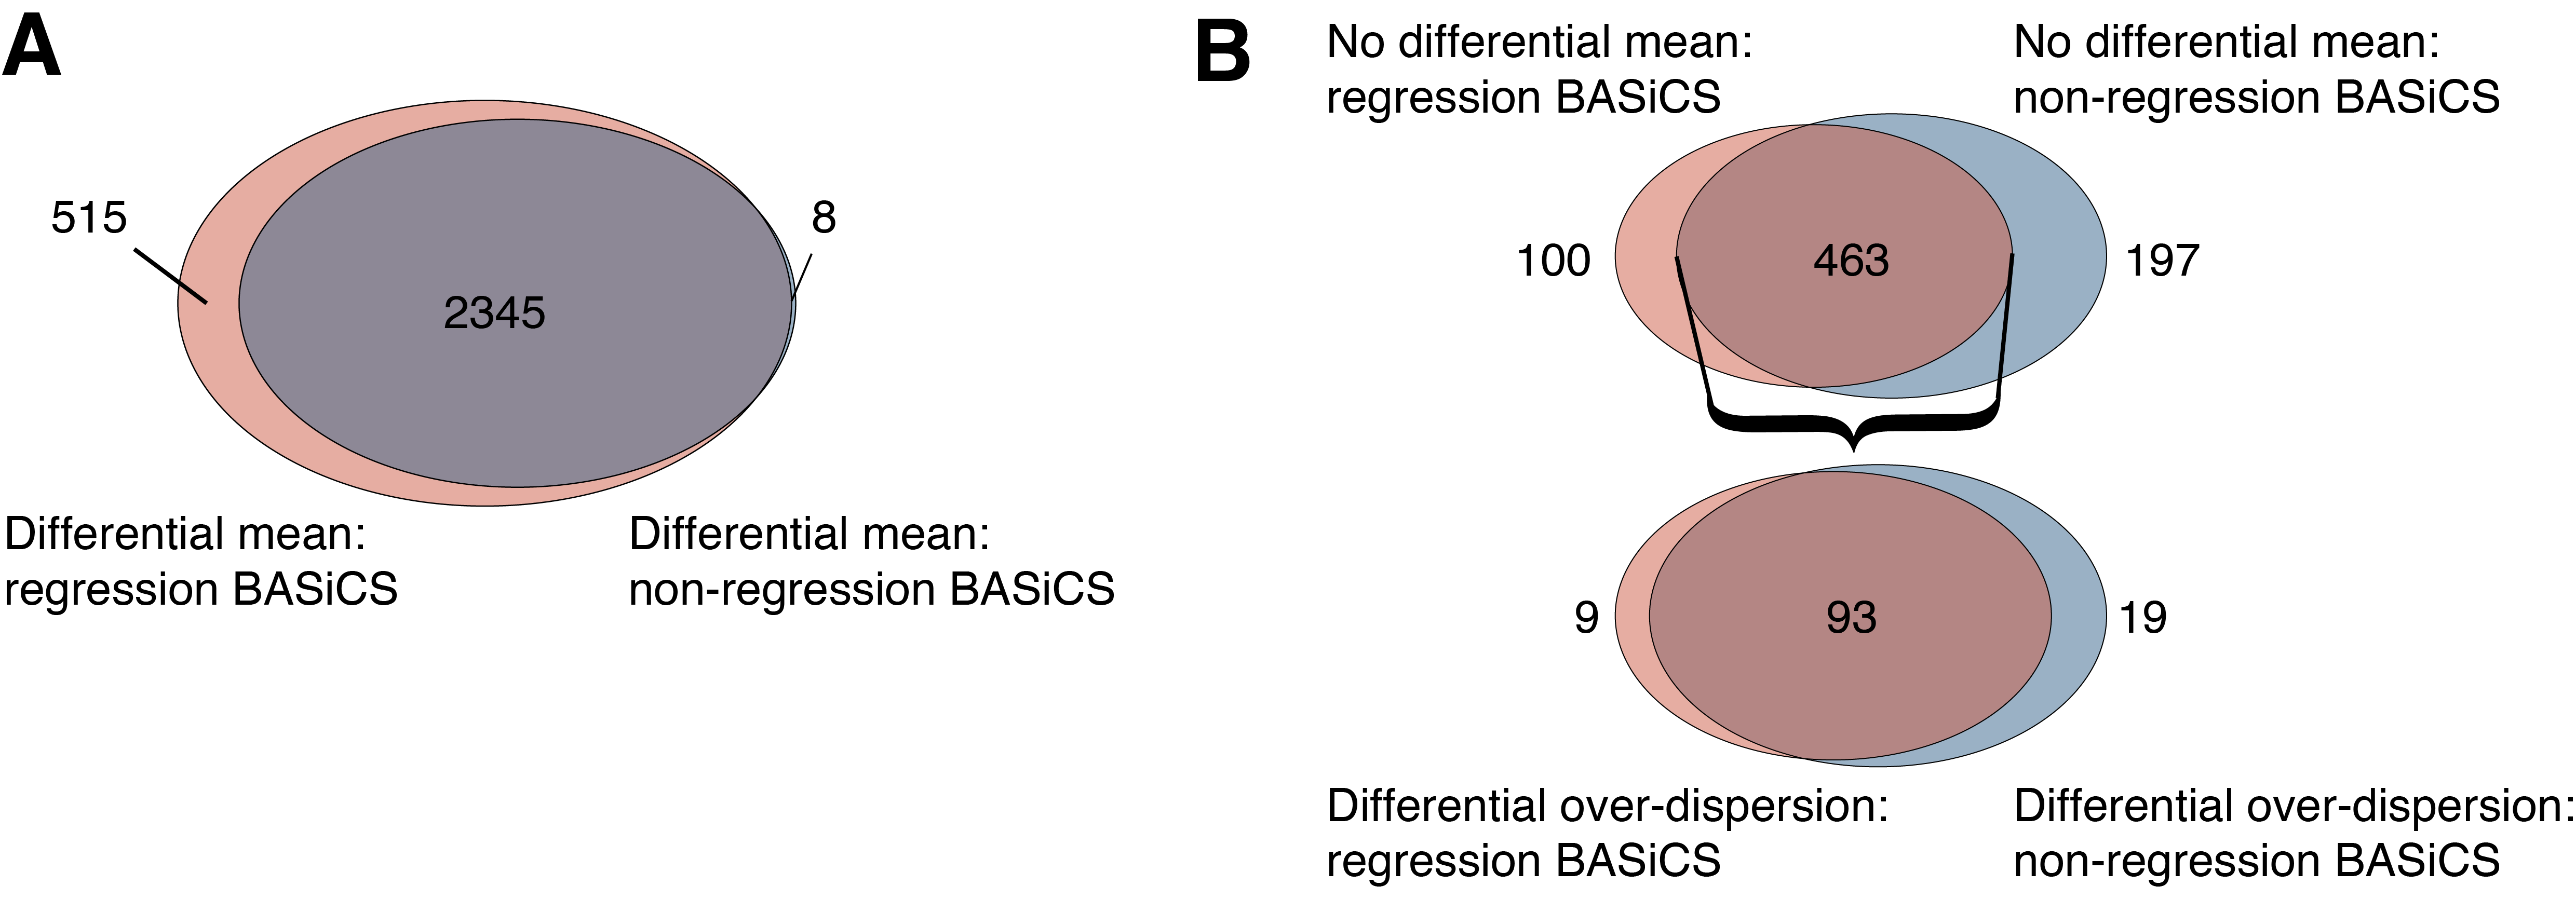
\includegraphics[width=\textwidth]{Fig_9.png}
\caption[Post-transcriptional regulation to control noisy expression]{\textbf{Post-transcriptional regulation to control noisy expression.}\\
Bursty expression introduces nuclear variation in transcript abundance that is buffered due to retention at the nuclear membrane. Within the cytoplasm, micro RNAs degrade lowly expressed genes to reduce expression noise. 
Deletion of the ribsosome binding site as well as stem loop formation increase variability in protein abundance across cells. 
Arrows indicate either increased (red) or decreased noise (green) depending on the regulatory mechanism.}
\label{fig0:posttranscriptional}
\end{figure} 

\newpage

Within the cytoplasm, mRNAs are subject to translation or degradation. 
At this stage, \cor{variability induced by} bursty gene expression is propagated to form variation in protein abundance. 
The availability of mRNAs for translation is not only dictated by their synthesis but also their degradation rate. 
mRNA degradation is accelerated by recognition of \glspl{miRNA}. 
This process has been shown to preferentially reduce noise levels for lowly expressed genes in mESCs, possibly to retain cellular identity \textbf{(Fig.~\ref{fig0:posttranscriptional})} \citep{Schmiedel2015}. 
\\

In addition to noise introduced by stochastic processes on the transcriptional level, the recognition and binding of ribosomes to mRNAs for translation initiation is a source for variation in protein abundance. 
Modulating translational efficiency by mutating the ribosome binding site and initiation codon showed an association between translation and variation in protein abundance \textbf{(Fig.~\ref{fig0:posttranscriptional})} \citep{Ozbudak2002}. 
Additionally, mRNA secondary structure formed by stem loops and poly(G) motifs affects translation initiation and increases variation in protein levels \textbf{(Fig.~\ref{fig0:posttranscriptional})} \citep{Dacheux2017a}.\\

\cor{Together, these studies again highlight a multitude of factors that can modulate the observable variation in transcript and protein abundance. 
Moving forward, models that correct or account for variations introduced by different factors need to be developed to disentangle the individual sources of molecular variation.}

\subsection{Extrinsic noise}

\cor{Classically, extrinsic noise was described to arise from fluctuations in molecules that affect the global gene expression landscape of the cell\cite{Elowitz2002}.
Measuring extrinsic noise is only possible in bacterial populations that so not show fluctuations in cell states.
Nowadays, extrinsic noise is often described to arises from cells being in different regulatory states.}
Here, differences in cellular components introduce variation in mRNA and protein abundance. 
The presence of cell states in otherwise homogeneous populations is characterised by differences in metabolism, cell cycle, cellular volume, cell-to-cell and environmental signalling as well as cell density. 
It has been shown that extrinsic noise forms a major contribution to variation in gene expression and that transcript distributions can be predicted from the cellular state, population context and microenvironment \citep{Battich2015a}.
\cor{Being able to predict transcript abundance however indicates that extrinsic noise is not purely stochastic but might also contain deterministic components.}

\subsubsection{Cell cycle}

Cell cycle has been widely discussed to form a \cor{major} source of extrinsic noise \citep{Colman-Lerner2005, Newman2006}. 
In yeast populations, differences in transcriptional activities between the G1 and S/G2/M phases of the cell cycle lead to large-scale transcriptional heterogeneity across cell populations \textbf{(Fig.~\ref{fig0:extrinsic})} \citep{Zopf2013}. 
Under nutrient-poor conditions, growth rate is reduced and \cor{transcriptional variability} is elevated due to cells being in different cell cycle stages \citep{Keren2015}. 
Even under optimal growth conditions for mESCs (2i media), cell cycle related genes show strong heterogeneity in expression across the cell population \citep{Kolodziejczyk2015cell}. 
\cor{However, it is possible that unobserved regulatory mechanisms are in place to induce proliferation, which otherwise appears to occur random across a population of cells.}
When quantifying cell-to-cell variation, cell cycle induced extrinsic noise is often seen as unwanted variation and can mask more subtle transcriptional heterogeneity. 
Computational methods have been developed to correct for this confounding effect to enhance the underlying signal \citep{Buettner2015, Buettner2017}. 

\begin{figure}[!h]
\centering
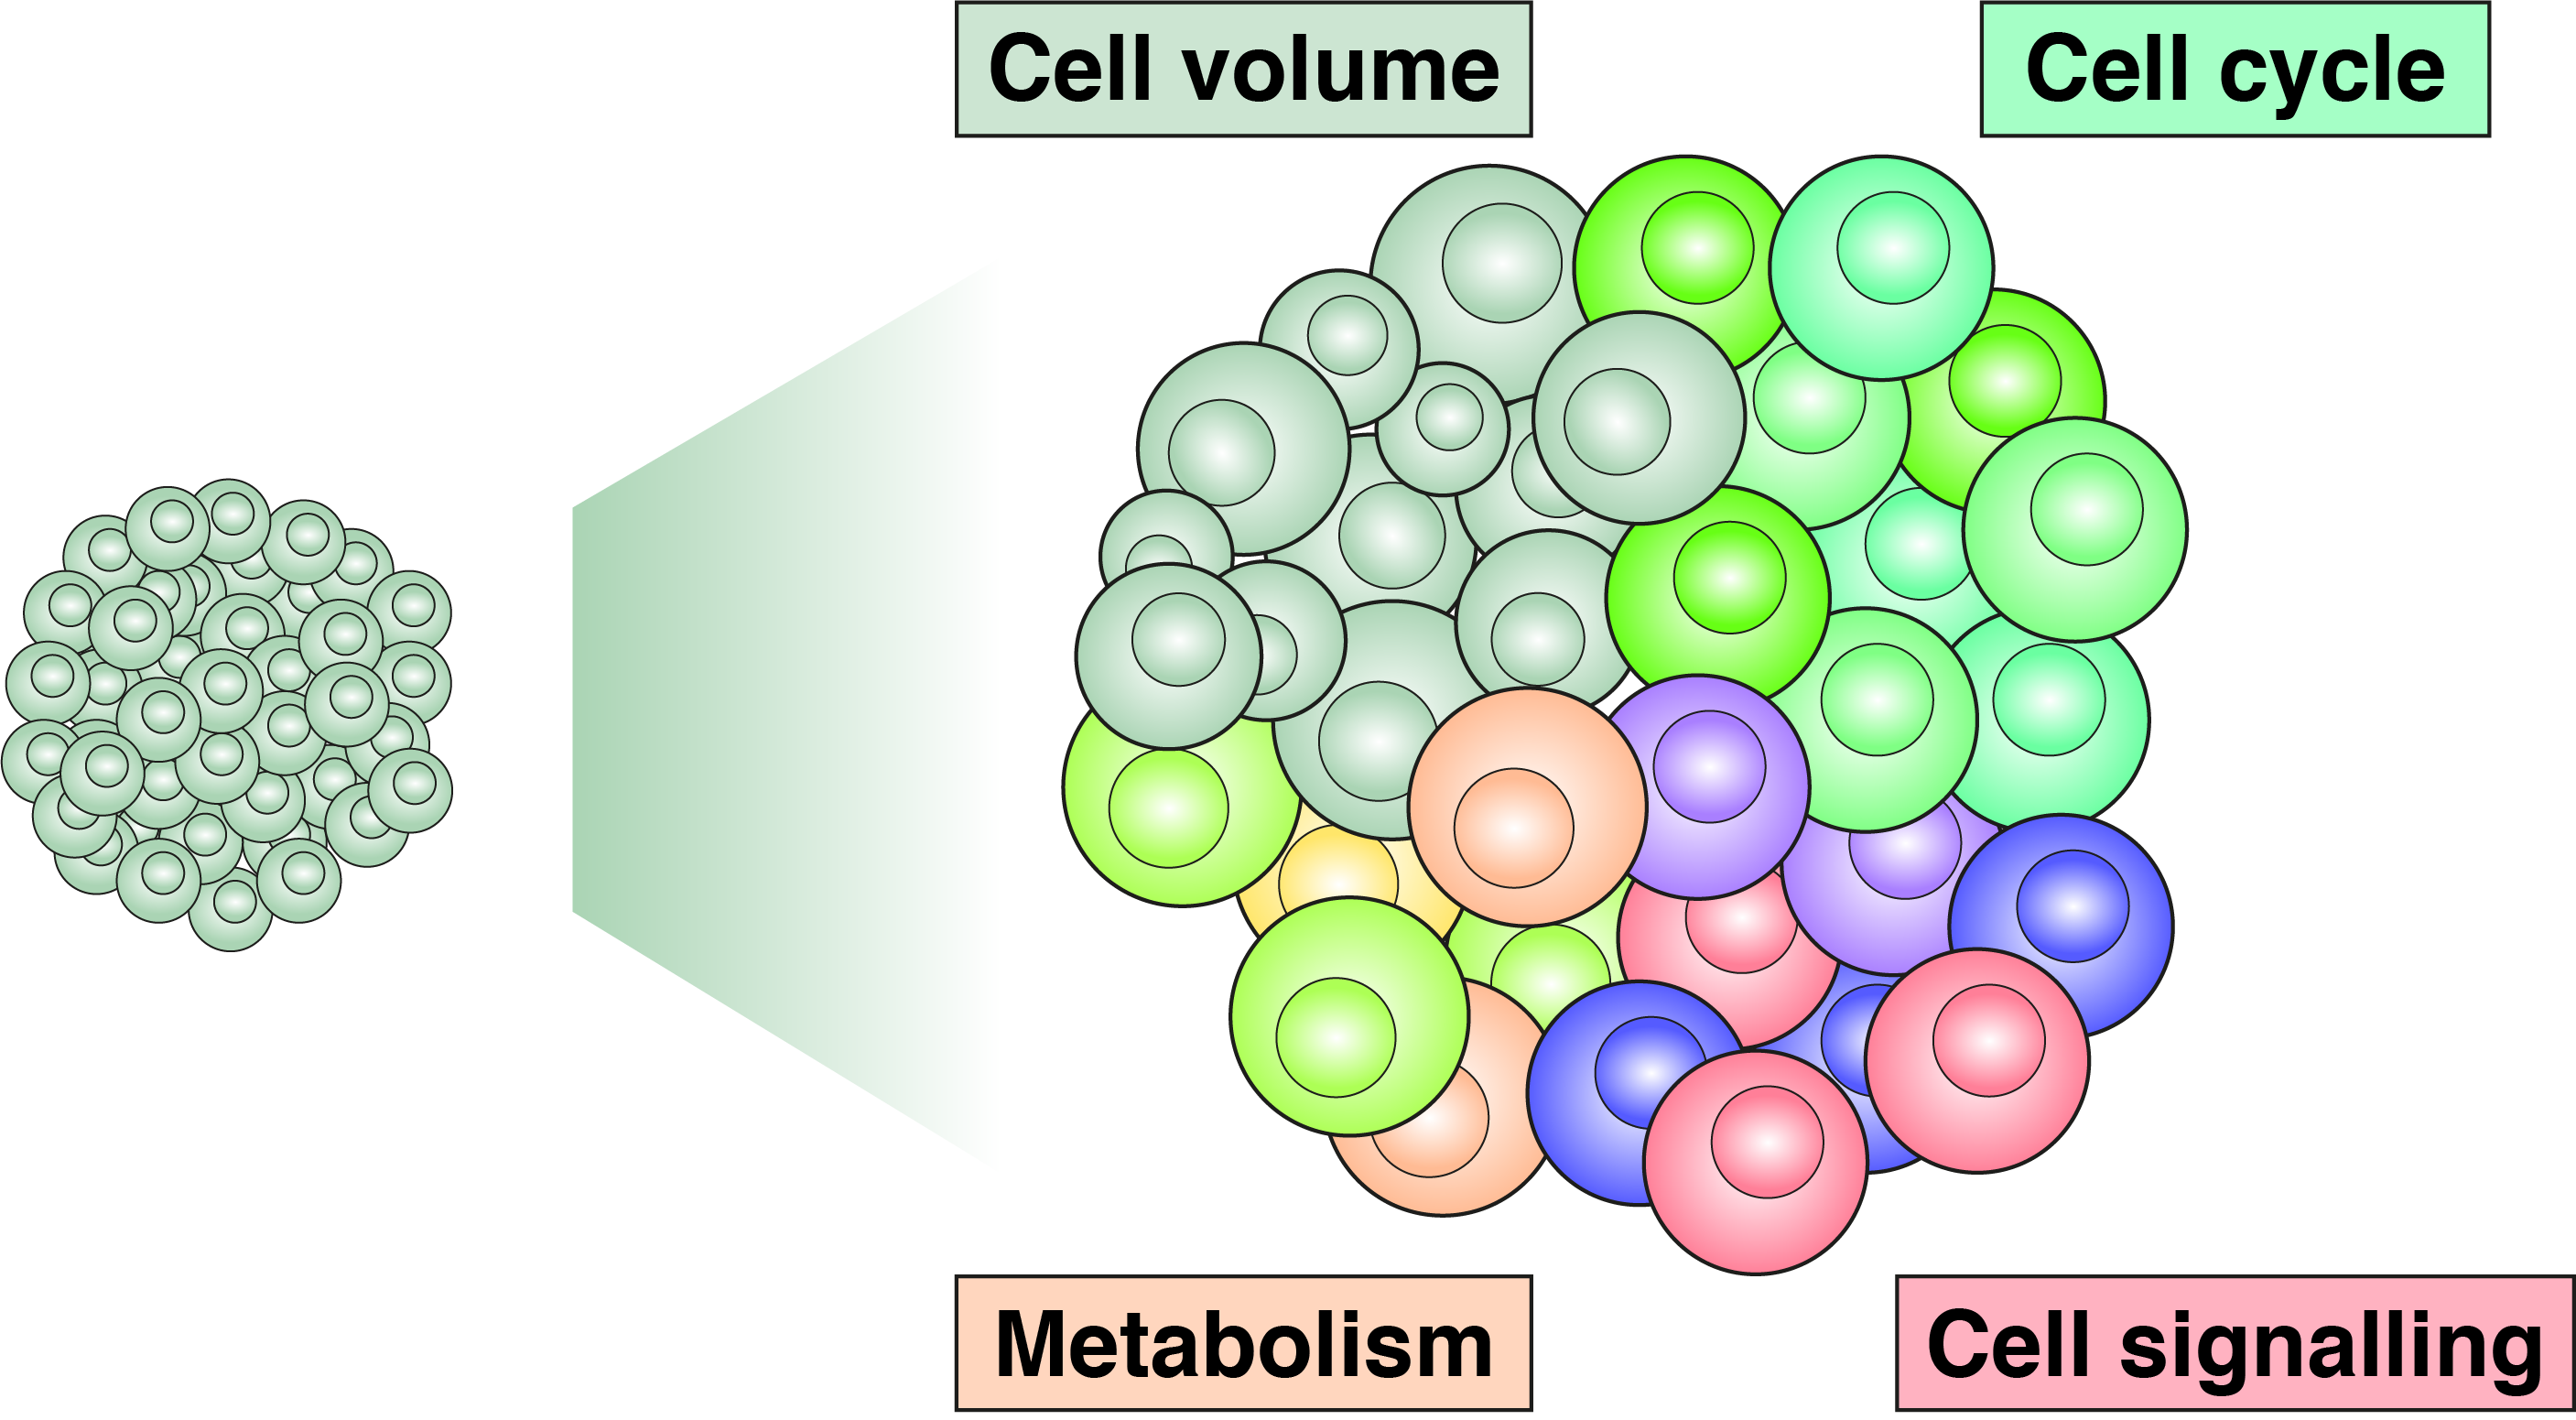
\includegraphics[width=0.7\textwidth]{Fig_10.png}
\caption[Differences in cell states induce extrinsic noise]{\textbf{Differences in cell states induce extrinsic noise.}\\
Within a homogeneous population of cells (left), individual cells reside in different cellular states (e.g.~cell cycle, cell signalling, metabolism) and show differences in cellular volume.}
\label{fig0:extrinsic}
\end{figure} 

\vspace{-5mm}

\subsubsection{Cell volume}

Cellular volume provides another explanation for global differences in mRNA content between individual cells introducing large-scale transcriptional \cor{variability} \textbf{(Fig.~\ref{fig0:extrinsic})}. 
Even though cell volume changes during cell cycle progression, within each phase, cell volume can vary as much as across all phases. 
It has been shown that mRNA counts scale with cellular volume to maintain transcript concentrations within each cell \citep{Kempe2015, Padovan-Merhar2015, Zhurinsky2010}. 
\cor{Again, it is not fully understood how cell volume is controlled across a population of cells; especially within multicellular organisms. 
Therefore, the volume of a cell does not necessarily stochastically but rather deterministically contribute to the observed molecular phenotypic variability.}
To avoid this source of heterogeneity, normalisation approaches correct for differences in mRNA content between individual cells \citep{Vallejos2017}.

\subsubsection{Metabolism}

The effect of metabolic fluctuations has been studied in \textit{E. coli} populations. 
Variations in biochemical reactions are induced by noise in the expression of their corresponding catalytic enzymes. 
Changes in metabolism are then coupled to varying growth rates of individual cells, which in turn introduce large-scale transcriptional heterogeneity in cell populations \textbf{(Fig.~\ref{fig0:extrinsic})} \citep{Kiviet2014}.  

\subsubsection{Expression capacity}

Expression capacity is defined as the ability of a cell to express proteins from a gene by utilising the transcriptional and translational machinery. 
Fluctuations in the expression capacity of cells due to quantitative differences in RNAPII or ribosomes can induce global variability among the majority of proteins \citep{Colman-Lerner2005}.

\subsubsection{Cell signalling}

A different source of extrinsic noise is the intra- or inter-cellular signalling state of individual cells. 
Fluctuations in membrane bound or cytoplasmic proteins lead to inconsistent transmission of signalling stimuli as exemplified by variability in \gls{TRAIL}-induced apoptosis \citep{Spencer2009}. 
Similarly, variations of regulators in the \gls{ERK} signalling pathway introduce downstream variability in nuclear response \textbf{(Fig.~\ref{fig0:extrinsic})}. 
The degree to which nuclear ERK response varies depends on the position of the regulator in the topology of the signalling pathway \citep{Iwamoto2016}. 
In \textit{C. elegans}, perturbation of the Wnt signalling pathway displayed different degrees of variability in expression of the key Hox gene for Q neuroblast migration, \textit{mab-5}. 
It has been proposed that extrinsic noise, in this case the strength of the Wnt signal, modulates intrinsic variation in the expression of \textit{mab-5} \citep{Ji2013}. 
\cor{These examples describe a system where noise introduces variation in individual components. 
However, this variation is modulated by signalling networks, which allows the cells to precisely respond to external cues. }

\subsubsection{Physical constraints}

\begin{wrapfigure}{r}{0.5\textwidth}
\centering    
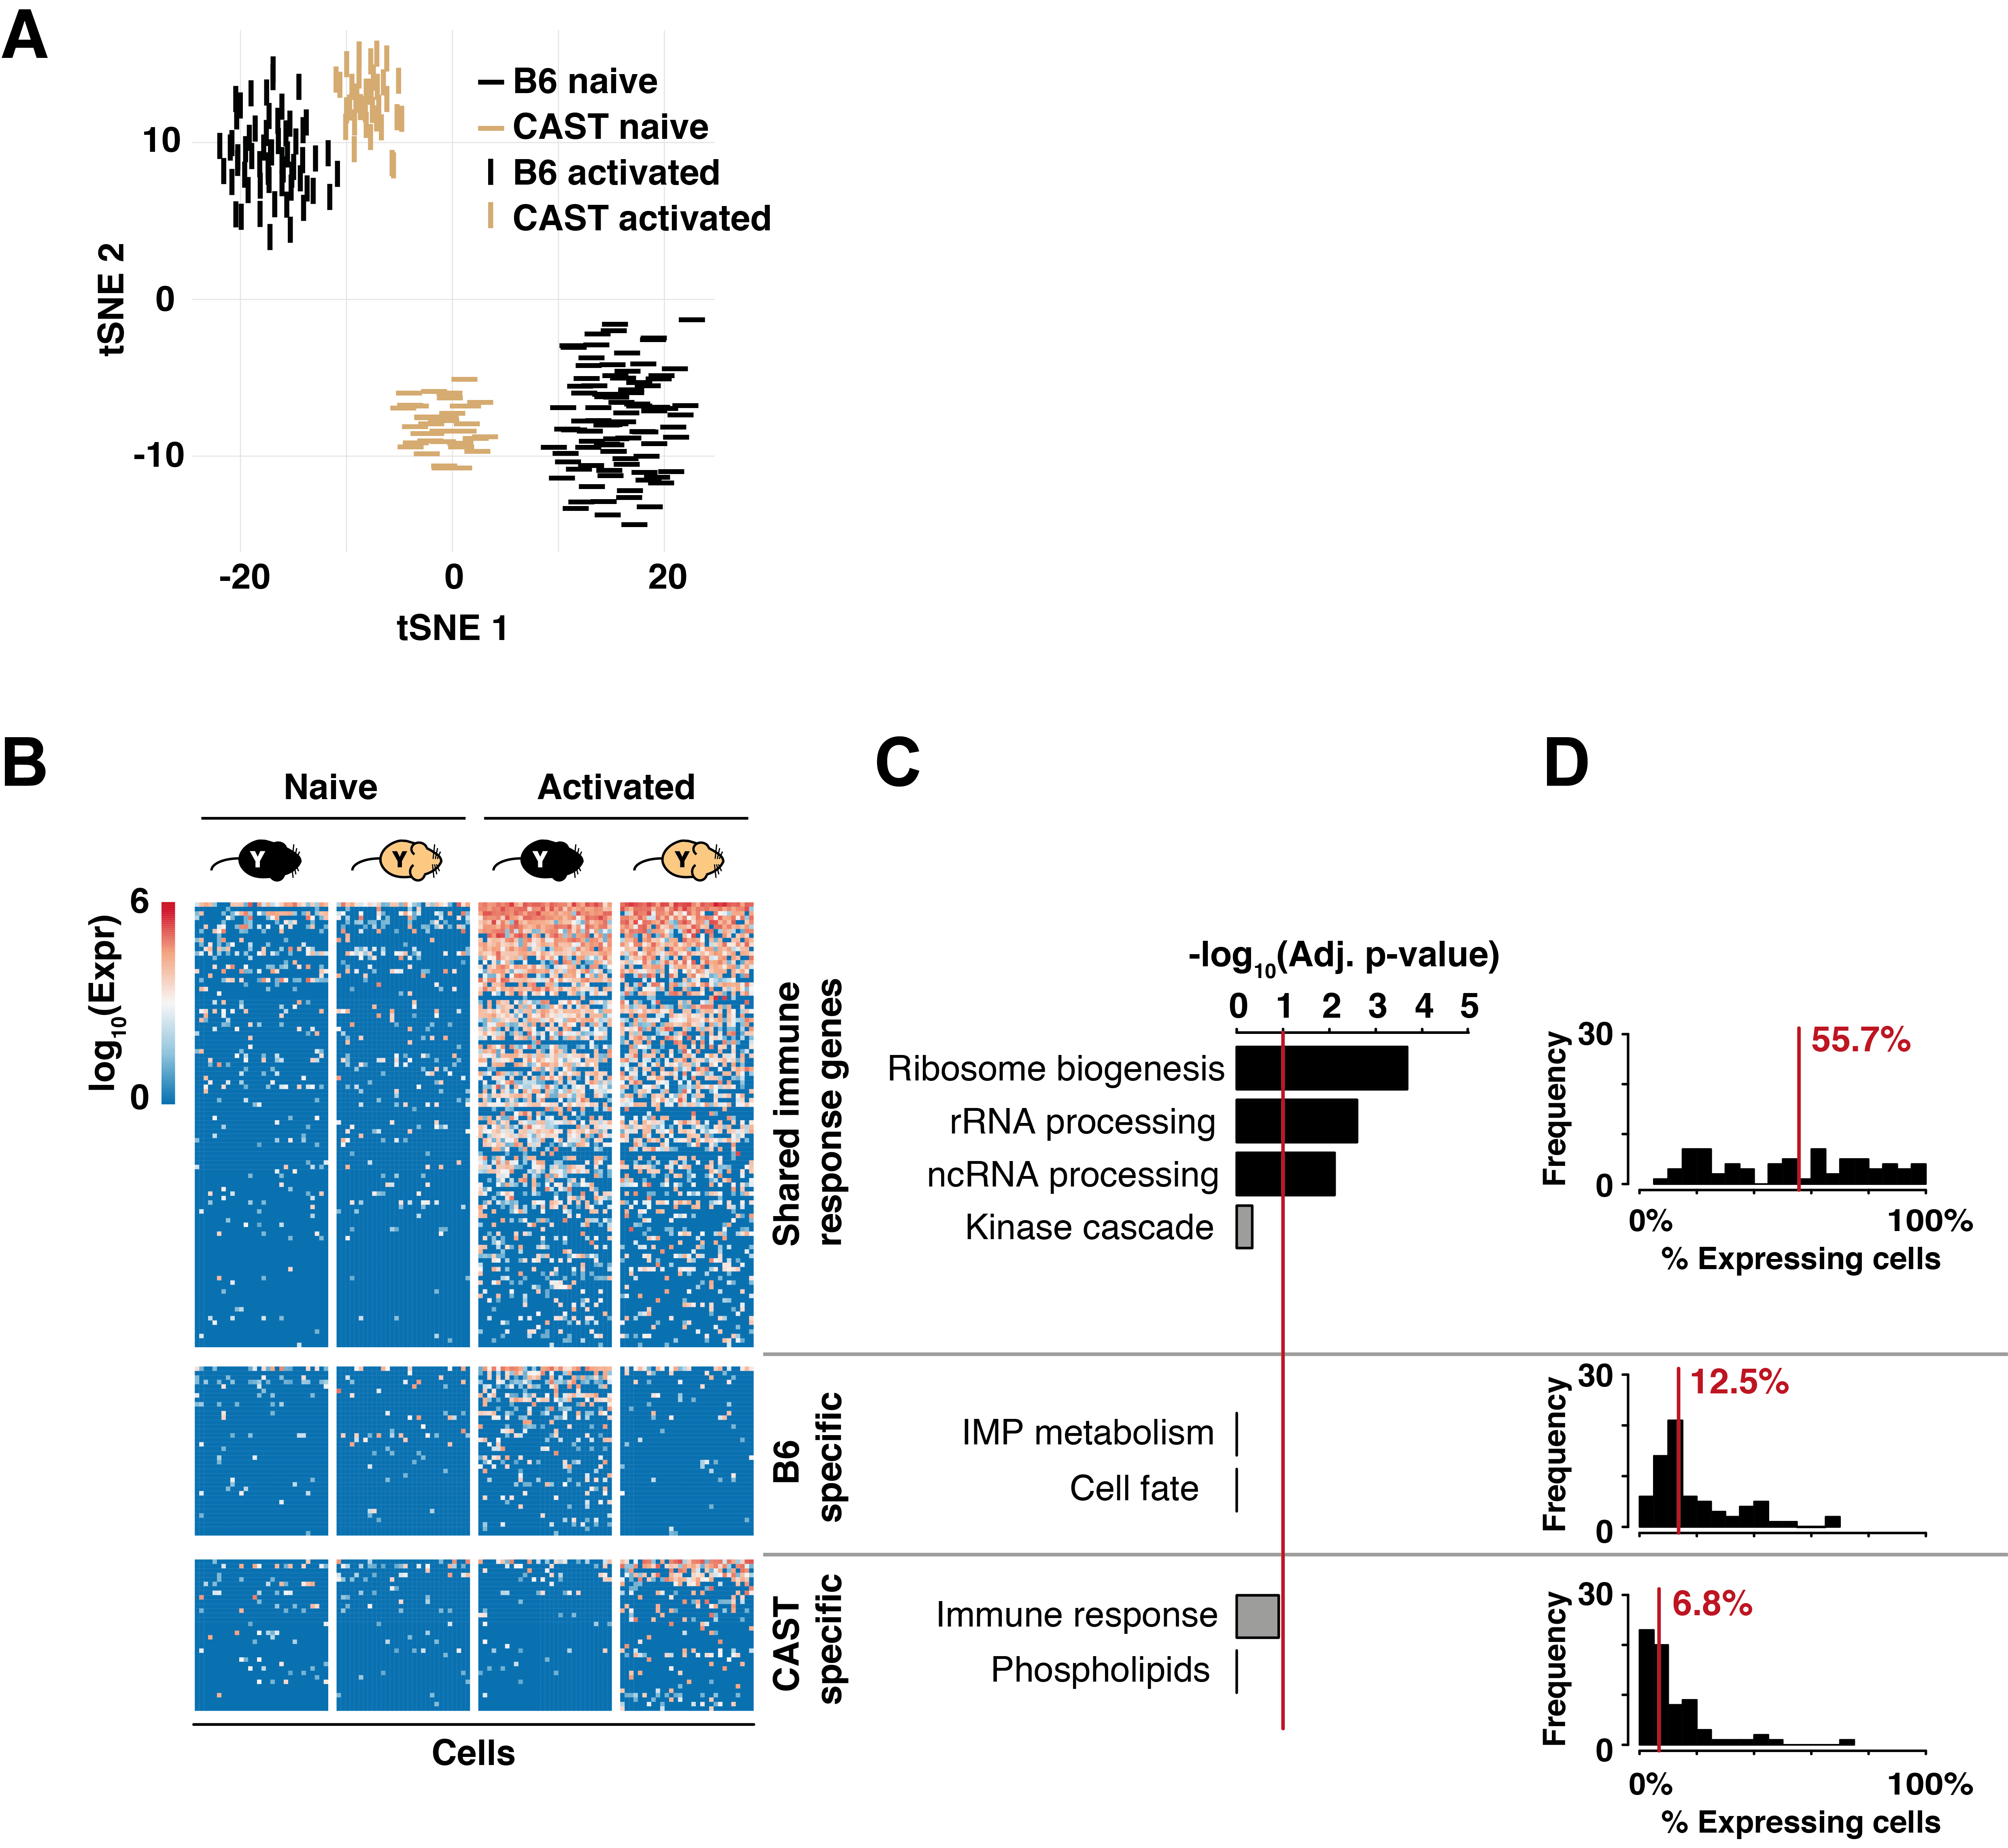
\includegraphics[width=0.48\textwidth]{Fig_11.png}
\caption[Physical constraints induce heterogeneous expression patterns.]{\textbf{Physical constraints induce heterogeneous expression patterns.} \\
Cell density increases during the expansion of a homogeneous population of cell forming patches with high and low density, pushing cells to the edge of the population. 
Based on these physical constraints, cells change their transcriptional programme, inducing variability across the population.}
\label{fig0:constrains}
\end{wrapfigure}

Physical constraints on cell growth and the direct population context influence the state of individual cells \citep{Battich2015a}. 
Snijder \textit{et al.}, 2009 performed detailed imaging based analysis of adherent human cells that were infected with different viruses. 
Clathrin mediated endocytosis was most variable with low cell density leading to inefficient mouse hepatits virus infection. 
Dengue virus preferentially infects edge cells while simian virus 40 infection decreased with large cell density \citep{Snijder2009}. 
These experiments indicate the importance of local cellular microenvironment and cell-cell contacts leading to heterogeneity in cell states \textbf{(Fig.~\ref{fig0:constrains})}. 

